\documentclass{article}
\input{C:/Users/aryay/OneDrive/Shared Files/Programs/Preamble.tex}


\title{Curvature Flow}
\author{Arya Yae}
\date{}

\begin{document}

\maketitle

\section*{Flow on a Disk}
The two standard real coordinate systems on $\R^2$ are $(x,y)$ and $(r,\theta)$, and there is also a single complex coordinate given by $z=x+iy$, and another given by $\bar z=x-iy$.  These are related as follows:
    $$(r,\theta)=(\sqrt{x^2+y^2},\arctan(y/x)),\qquad (x,y)=(r\cos\theta,r\sin\theta),$$
    $$z=re^{i\theta},\qquad \bar z=re^{-i\theta}.$$
The operators $\partial_x=\frac{\partial}{\partial x}$, etc.\ can be thought of as vectors, so that $\partial_x f$ represents the change in $f$ in the direction of the vector $\partial_x$.  Using some differential geometry, we have the following relationships:
    $$\partial_z=\frac12(\partial_x-i\partial_y),\qquad \partial_{\bar z}=\frac12(\partial_x+i\partial_y),$$
    $$\partial_z=\frac{e^{-i\theta}}{2r}(r\partial_r-i\partial_\theta),\qquad \partial_{\bar z}=\frac{e^{i\theta}}{2r}(r\partial_r+i\partial_\theta).$$
The standard laplacian is $\Delta=\partial_{xx}+\partial_{yy}$.  By composing the above formulas and (using the product rule), we can also write
\begin{align}
    \Delta
        &=4\partial_{\bar z}\partial_z,\\
        &=\partial_{rr}+\frac1r\partial_r+\frac1{r^2}\partial_{\theta\theta}.
\end{align}
Based on our experience so far, it seems like polar coordinates are best for curvature flow and complex coordinates are best for calculating geodesics.

The \emph{standard metric} $g_0$ can be expressed as $g_0=(\de x)^2+(\de y)^2$ or $g_0=(\de r)^2+r^2(\de\theta)^2$ or $g_0=|\de z|^2$.  This is technically called a \emph{symmetric $(0,2)$-tensor}, but as far as we are concerned it simply represents the method being used to measure the (squared) length of vectors.

Associated to $g_0$ is the \emph{standard symplectic form} $\omega_0=\de x\wedge\de y$ or $\omega_0=\frac1{2i}\de\bar z\wedge\de z$ or $\omega_0=r\,\de r\wedge\de\theta$, which is an \emph{antisymmetric $(0,2)$-tensor} used to measure the area of parallelograms.  These are mostly used for integration.

As in the stereographic projection example, we often want to use portions of $\R^2$ to represent patches of a surface which has different geometry.  This makes the notion of distances between points vary depending on the location in $\R^2$.  Thus, we can used a positive \emph{weight function} $u$ on $\R^2$ to create a new metric $g=ug_0$ (see \Cref{fig: Stereographic Projection}).  In the various coordinate systems this looks like\footnote{It is commonplace to use $\de x^2$ to denote $(\de x)^2$; this should not be confused with $\de(x^2)$.}
\begin{align}
    g
        &=u(x,y)\,(\de x^2+\de y^2)\\
        &=u(r,\theta)\,(\de r^2+r^2\de\theta^2)\\
        &=\frac1{2i}u(z)\,|\de z|^2.
\end{align}
The associated symplectic form is $\omega=u\,\omega_0$.  When doing curvature flow, this weight function $u$ is what evolves over time.  Some, such as Jost, use $\lambda^2$ in place of $u$ to avoid worrying about negative values.  However Mazzeo-Rubinstein-Sesum just use $u$.

\begin{figure}
    \centering
    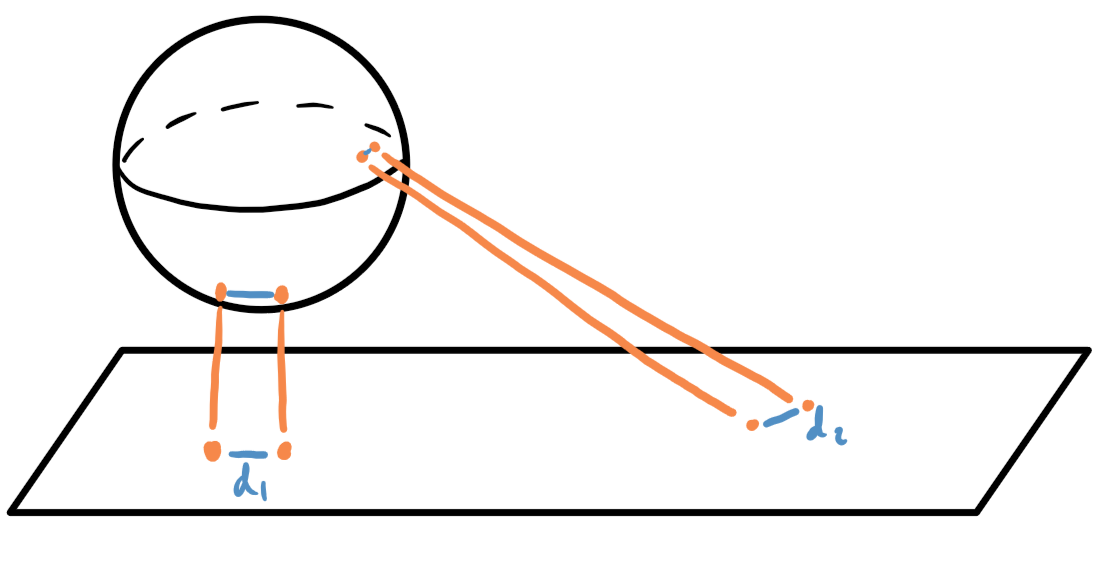
\includegraphics[width=.5\textwidth]{stereographic_projection.png}\qquad
    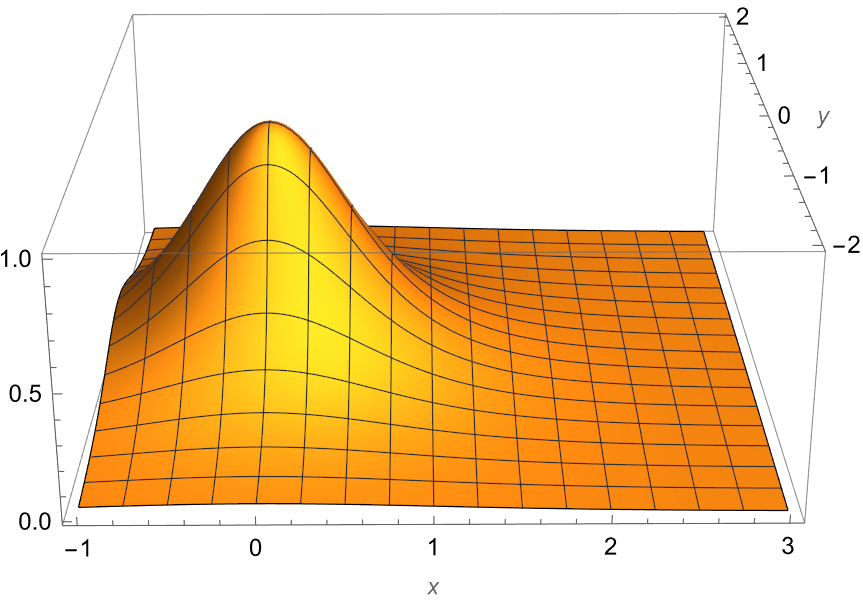
\includegraphics[width=.4\textwidth]{fubini_study_metric.png}
    \captionsetup{width=.9\textwidth}
    \caption{The image on the left is the stereographic projection, wherein the metric should measure $d_1$ as larger than $d_2$.  Thus, the weight function $u$ should be smaller away from the origin in $\R^2$.  This is reflected in the image on the right, which shows the graph of the weight function for the Fubini-Study metric.}
    \label{fig: Stereographic Projection}
\end{figure}

\begin{definition*}
    Given a metric $g=ug_0$, the \emph{metric laplacian} is $\Delta_g=\frac1u\Delta$ where $\Delta$ is the standard laplacian, and the \emph{scalar curvature} is $K_g=\Delta_g\log u$.
\end{definition*}

The reason for the $\frac1u$ factor has to do with coordinate changes.  To illustrate this, consider the act of ``zooming in'' to a point on the sphere, which makes the curvature appear `flatter.'  The formula $\Delta\log u$ will reflect this fact, which is undesirable because we want the curvature to be a fixed number independent of what coordinates we are using.  Using $K_g=\Delta_g\log u=\frac1u\Delta\log u$ accounts for this.

Note that $K_g$ is a function on $\R^2$, because the curvature depends on the location.  The purpose of Ricci flow is to even out the curvature, to make $K_g$ a constant function.  The limit is called a \emph{uniformization metric}.

Let $g_t=u_tg_0$ be a family of metrics\footnote{The $t$ subscript does not mean derivative.  We'll stick with $\partial$ notation for derivatives.}, and let $K_t=K_{g_t}$.  Let $U\subseteq\R^2$ be a region.  With respect to the metric $g_t$, the volume (area) of $U$ is $\mathrm{Vol}_t(U)=\int_U \omega_t=\int_U u_t\,\de x\,\de y$ and the average curvature on $U$ is
    $$\rho_t=\frac1{\mathrm{Vol}_t(U)}\int_U K_t\omega_t=\frac1{\mathrm{Vol}_t(U)}\int_U K_tu_t\,\de x\,\de y.$$

The \emph{normalized Ricci flow equation} on $U$ is
\begin{equation}
    \partial_tg_t=(K_{g_t}-\rho_t)g_t.
\end{equation}
The left hand side is $\partial_t(u_tg_0)=(\partial_t u_t)g_0$ and the right hand side is $(\frac1{u_t}\Delta\log u_t-\rho_t)u_tg_0$, so the above equation simplifies to
\begin{equation}
    \partial_tu_t=\left(\frac1{u_t}\Delta\log u_t-\rho_t\right)u_t.
\end{equation}

Now let $D\subseteq R^2$ be the unit disk and let $S$ be the boundary.  Given an initial weight function $u_0$ and boundary function $u_t\big|_S=f$ for all $t$, we can perform Ricci flow on the disk.  If we remove the term $\rho_t$ we get the unnormalized Ricci flow $\partial_tu_t=\Delta\log u_t$, and by fixing a constant value $\rho$ we obtain the Yamabe flow which can flow the metric to one of constant curvature $\rho$, meaning $K_t$ approaches a constant function $\rho$.  However, both unnormalized Ricci flow and Yamabe flow have a tendency to diverge under certain conditions.


\section*{Tasks}
\noindent
\textbf{Task 1:}
Let the initial condition be $u_0=1$ and let the boundary condition be $f=1$.  Set $\rho=1$.  Perform Yamabe flow to approximate the uniformization metric with curvature $\rho$.  Then try various other values of $\rho$.

\noindent
\textbf{Task 2:}
Attempt a similar Yamabe flow when the boundary condition is not radially symmetric.

\noindent
\textbf{Task 3:}
Once we solve Task 1, we can plot geodesics for various $t$ values, each with the same initial point and velocity.

\noindent
\textbf{Task 4:}
The solution to Task 1 should converge to the Fubini-Study metric, which has weight function $u=\frac1{(1+|z|^2)^2}$.  This is the behavior on the ``south pole chart'' of the sphere.  Using the mapping $w=\frac1z$ from the south pole chart to the north pole chart to glue together two copies of the initial conditions from Task 1, perform \emph{normalized Ricci flow} on the whole sphere.


\end{document}